% Standalone vector figure. Build with xelatex.
\documentclass[tikz,border=3pt]{standalone}
\usepackage{fontspec}
\setsansfont{texgyreheros-regular.otf}[BoldFont=texgyreheros-bold.otf]
\usepackage{amsmath,unicode-math}
\setmathfont{texgyretermes-math.otf}
\usetikzlibrary{arrows.meta}
\definecolor{ink}{HTML}{24374B}
\definecolor{line}{HTML}{8291A1}
\definecolor{pale}{HTML}{F3F6F9}
\newcommand{\matmul}{\mathbin{@}}
\begin{document}
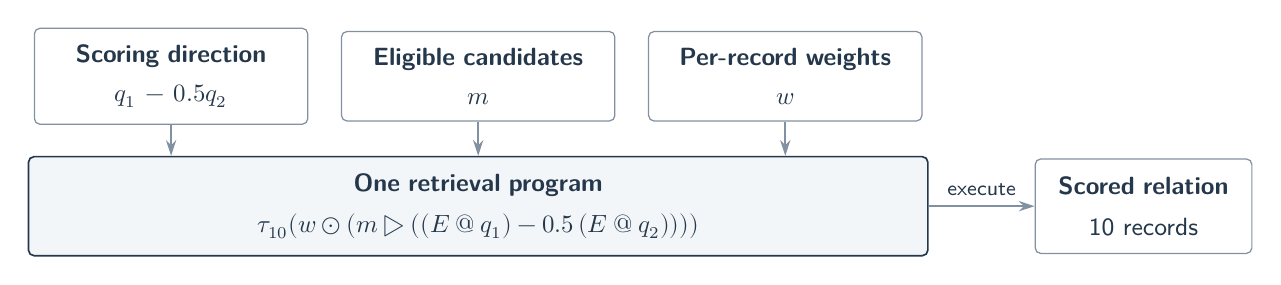
\begin{tikzpicture}[
  font=\sffamily\fontsize{9}{11}\selectfont,
  text=ink,
  choice/.style={draw=line,fill=white,rounded corners=2pt,
    line width=0.45pt,text width=3.05cm,minimum height=1.0cm,
    inner sep=6pt,align=center},
  program/.style={draw=ink,fill=pale,rounded corners=2pt,
    line width=0.6pt,text width=11.0cm,minimum height=1.2cm,
    inner sep=6pt,align=center},
  result/.style={draw=line,fill=white,rounded corners=2pt,
    line width=0.45pt,text width=2.4cm,minimum height=1.2cm,
    inner sep=5pt,align=center},
  flow/.style={-{Stealth[length=2mm,width=1.3mm]},draw=line,line width=0.65pt}
]
\node[choice] (direction) at (1.85,1.65)
  {\textbf{Scoring direction}\\[3pt]\(q_1-0.5q_2\)};
\node[choice] (mask) at (5.75,1.65)
  {\textbf{Eligible candidates}\\[3pt]\(m\)};
\node[choice] (weight) at (9.65,1.65)
  {\textbf{Per-record weights}\\[3pt]\(w\)};
\node[program] (query) at (5.75,0)
  {\textbf{One retrieval program}\\[4pt]
   \(\displaystyle
     \tau_{10}\!\left(
       w\odot\left(m\triangleright
         \left((E\matmul q_1)-0.5\,(E\matmul q_2)\right)
       \right)
     \right)
   \)};
\node[result] (output) at (14.2,0)
  {\textbf{Scored relation}\\[4pt]10 records};
\draw[flow] (direction.south) -- (direction.south |- query.north);
\draw[flow] (mask.south) -- (query.north);
\draw[flow] (weight.south) -- (weight.south |- query.north);
\draw[flow] (query.east) -- node[above,font=\sffamily\fontsize{7.5}{9}\selectfont]
  {execute} (output.west);
\end{tikzpicture}
\end{document}
